% STOA @ PVLDB (Workload Characterization / EA&B track).
% Template: the official VLDB-Template bundle (github.com/vldbproceedings/VLDB-Template),
%   which pins acmart.cls v2.19 and layers pvldb.sty on top. Both are vendored here so the
%   build does not depend on the local TeX install's acmart version.
% CfP constraints (verified 2026-08-12, vldb.org/2027/submission-guidelines.html):
%   deadline 1st of each month 5PM PT, abstract mandatory by the 25th of the prior month
%   12 pages EXCLUDING references | EA&B papers must link a reproducibility package
% Build: pdflatex main && bibtex main && pdflatex main && pdflatex main
% The previous CIDR-formatted version is preserved as main_cidr.tex.
\documentclass[sigconf, nonacm]{acmart}
%%% do not modify the following VLDB block %%
%%% VLDB block start %%%
\usepackage{pvldb}
%%% VLDB block end %%%
\renewcommand\vldbdoi{XX.XX/XXX.XX}
\renewcommand\vldbpages{XXX-XXX}
\renewcommand\vldbavailabilityurl{https://github.com/ANONYMIZED/stoa}

\let\Bbbk\relax        % avoid clash: acmart's newtxmath already defines \Bbbk
\usepackage{amssymb}   % for \checkmark in Table 1
\usepackage{makecell}
\usepackage{multirow}
\usepackage{cleveref}
\graphicspath{{figs/}}
\setlength{\footskip}{12pt}

% --- Citation-key map (verified against docs/references.bib) ---
% memos=F1_li2025memos  memgpt=P14_packer2023memgpt  memoryr1=F6_yan2025memoryr1
% memaction=F7_zhang2025memoryasaction  lmcache=F5_liu2025lmcache  mplus=F2_wang2025mplus
% sleeptime=F3_lin2025sleeptime  lightmem=F4_fang2025lightmem  raggym=F20_xiong2025raggym
% parrot=S2_liu2020parrot  decima=S5_mao2019decima  coldrl=S4_coldrl2025  h2o=S1_zhang2023h2o
% locomo=P51_maharana2024locomo  longmemeval=P52_wu2025longmemeval  memoryagentbench=F46_hu2025memoryagentbench

\begin{document}

\title{Ranking Is Not Placement: What Production KV Traces Say About Learned Memory Tiering}
\subtitle{A budget-constrained formulation, a decoupling result, and the protocol that found it}

\author{STOA Project}
\affiliation{%
  \institution{Semyung University}
  \city{Jecheon}
  \country{Republic of Korea}}
\email{suanlee@semyung.ac.kr}

\begin{abstract}
LLM agents increasingly depend on external memory, and the decision that governs it---for each memory
item, in what \emph{representation}, on which \emph{storage tier}, and \emph{when} to (re)materialize
it---is today split across three communities that each optimize one axis and fix the others. We argue
these axes are \emph{coupled} and give a single budget-constrained MDP over
representation~$\times$~tier~$\times$~timing with one serve-time $(L,C,B)$ knob. We then ask the
empirical question the framing invites: is the decision learnable? On two production KV-trace sources we
find a decoupling rather than an answer in either direction. Reuse is predictable, and more so the longer a
block has been observed---ranking whether a block will be reused reaches AUC 0.93 at full trace
length---but across a length sweep in which both traces are run to exhaustion, the placement benefit that buys stays inside
$[+0.8\%, +2.9\%]$ of an 81--87\% gap to a hindsight oracle and does not trend with ranking quality. Three
controls locate the reason: rank-normalizing beliefs barely moves the outcome, so ordering is the
operative mechanism; substituting true future counts recovers 95\% of the gap, so the placement
machinery is not the bottleneck; and a capacity ladder from a linear model through boosted trees to a
neural network lands within 0.4 points of itself on placement despite a 13-point spread in their AUC, so
neither is the hypothesis class. Tiering rules that forecast nothing at all --- LRU, LFU, a fill-once cache --- reach 75--99\% of Belady
on one trace and 40--94\% on the other, and the whole adaptive-replacement family --- ARC, LeCaR, CACHEUS
and a reimplementation of LRB --- beats the best plain rule by at most 4.6 points of Belady across eight
operating points, and at two of them by nothing. They share one failure mode: 76--78\% of blocks are
never reused, which leaves the adaptive policies a signal on 3.5--7.3\% of misses and right-censors
77--83\% of the learned one's training rows. On LoCoMo, re-run at the size a power analysis asked for --- ten dialogues, 300 scored questions per
arm, paired tests --- query-aware retrieval beats query-agnostic placement by a factor of four at a tight
budget in 10 of 10 dialogues, while the placement signal still beats embedding centrality within its own
regime: the two compose rather than compete. Exercising the representation axis for the first time
points \emph{against} our own framing --- one representation leads at every budget instead of crossing,
though at $n{=}100$ per cell that is a direction, not yet a result. We report the protocol this took as a first-class result: ten measurement
defects, six of them reference-frame mismatches and three extrapolations from a single value of a
parameter fixed for convenience. One of those reversed a headline claim from $+88\%$ to $-48\%$ when
swept, and randomizing the sample it was drawn from --- a control costing minutes --- put four draws
between $-234$ and $+66$ points, a spread an order of magnitude wider than the effect. It had never been
a measurement.
\end{abstract}

\keywords{LLM agents, agent memory, memory tiering, learned scheduling, budget-constrained MDP}

\maketitle

%%% VLDB block start %%%
\vldbtopmatter
%%% VLDB block end %%%

\section{Introduction}
\label{sec:intro}

Large language model (LLM) agents increasingly depend on memory that outlives a single context
window---the facts they extract, the turns they have seen, the tools they have run, the summaries they
have written. How well an agent answers, how fast it responds, and how much it costs are all decided by
one question asked of every memory item: \textbf{in what form should it be kept, where should it live,
and when should it be (re)materialized?} Concretely, each item can be stored as plaintext, a vector, a
graph, a latent/KV activation, or baked into parameters; it can sit on GPU, CPU, disk, or a remote tier;
and it can be written inline while serving, consolidated during an idle window, or left untouched.

Today this single decision is \textbf{fragmented across three research communities}, each of which
optimizes one axis and freezes the others. Memory-operating-system work---MemOS~\cite{F1_li2025memos},
MemGPT~\cite{P14_packer2023memgpt}---provides the primitives to migrate an item between representations
and tiers, but \emph{decides when to migrate by hand-tuned heuristics}. Reinforcement-learned memory
managers---Memory-R1~\cite{F6_yan2025memoryr1}, Memory-as-Action~\cite{F7_zhang2025memoryasaction}---learn
\emph{what content} to add, update, or delete, but operate over a single fixed representation and never
choose a tier or schedule an offline write. Systems-level cache tiering---LMCache~\cite{F5_liu2025lmcache}%
---places bytes across GPU/CPU/disk/remote to minimize \emph{miss rate or time-to-first-token}, with no
notion of the downstream task utility that the memory actually serves.

Our central observation is that \textbf{these three axes are coupled and cannot be optimized separately.}
Promoting an item to a latent or parameter representation is an expensive offline write, but it is then
cheap and fast to serve; leaving it as plaintext on disk is cheap to write but slow to read and heavy on
context tokens. The best representation depends on the tier and on how often the item will be reused; the
best tier depends on the representation's serving cost and the item's size; and whether to pay the
promotion cost at all depends on the budget. This is precisely a \textbf{budget-constrained scheduling
problem}---and a large body of ML-for-systems work (Belady-oracle imitation for cache
replacement~\cite{S2_liu2020parrot}, GNN schedulers for clusters~\cite{S5_mao2019decima}, offline-RL cache
eviction in production~\cite{S4_coldrl2025}) demonstrates that such problems are learnable.

The reason to act now is that every substrate exists but nothing orchestrates them: MemCube migration, RL
memory managers, tiered KV caches, latent memory~\cite{F2_wang2025mplus}, and sleep-time
consolidation~\cite{F3_lin2025sleeptime} all landed by late 2025, unconnected. What is missing is a
\emph{learned scheduler} that, per item and under a shared budget, trades accuracy against latency and
cost, with \textbf{task utility---not miss rate---as the objective.}

We present \textbf{STOA} (Storage \& Tiered Orchestration for Agents), a learned control plane that
decides \textbf{representation $\times$ tier $\times$ timing jointly}, per memory item, as a single
budget-constrained Markov decision process. The operator sets a latency/cost/token budget $(L,C,B)$ at
serving time and one policy adapts, tracing the accuracy--latency--cost frontier without retraining. To
tame the combinatorics (fifty legal actions per item, across many items) STOA factors the policy into
representation, tier, and timing heads over a graph network of the memory store, and evaluates it only
over the legal joint actions so masking is exact. It warm-starts the policy by imitating a Belady oracle
and assigns credit for delayed, query-time payoffs with a mix of oracle imitation and process
supervision~\cite{F20_xiong2025raggym}.

Having built the formulation, we take seriously the empirical question it invites---\emph{is this decision
actually learnable?}---and answer it on production KV traces rather than on synthetic workloads. The
answer turned out to depend less on the model than on \emph{when the model is asked}.

Placement studies of this kind, including three revisions of this one, fix a split instant: observe a
prefix, build features from it, place every block, and bill the result against the future. Feature
construction can only describe a block that has been seen --- and on these traces 45--46\% of blocks have
no pre-split access at all, while the hindsight oracle they are scored against ranks them anyway. Those
blocks carry \textbf{97\% of the oracle's advantage}. A policy confined to the remaining 3\% looks flat
however well it ranks, which is precisely what our earlier ``ranking does not convert into placement''
result measured. We retract it.

Moving the decision to each block's \emph{arrival} --- placing it the moment it first appears, from the
session context available at that instant --- raises the reachable share from 3\% to \textbf{83.5\%} on
one trace and 2\% to \textbf{19.0\%} on the other. What captures it is not prediction:
first-come-first-served admission with a fixed action reaches 87.4\% and 50.2\% of the ceiling, while a
learned arrival-time ranker at AUC 0.574 and 0.635 reaches 84.5\% and 47.2\% --- less, on both. But the
arrival \emph{order} is not free: shuffling it costs 3.3 points on one trace and \textbf{14.1} on the
other. So the design implication is narrower than ``deciding at all is enough'': build an
\textbf{admission point} rather than a predictor, and do not assume the order it admits in is
incidental.

Reaction is competitive for a related reason. Tiering rules that forecast nothing at all --- LRU, LFU and
a fill-once cache --- reach 75--99\% of Belady's hit rate on one Mooncake trace and 40--94\% on the other,
and the whole adaptive-replacement family (ARC, LeCaR, CACHEUS) beats the best of them by \emph{at most
4.6 points}. All of them adapt on a ghost hit, and 76--78\% of blocks here are never reused, so most
evictions are correct and emit no signal: ARC gets one on 3.5--7.3\% of misses. A population of
singletons starves the channel adaptive replacement runs on.

We report how much measurement discipline this took, because it is the part most likely to transfer, and
because it is not a flattering story. Three claims were retracted, the last two only under adversarial
review \emph{after} the error catalogue below had been written: a headline that randomized sampling
showed had never been measurable, the decoupling result above, and an LRB column that turned out to
measure random eviction because a training buffer was truncated to its tail. Two further sub-claims of
the present framing were falsified later still, by a re-verification pass run after this paper was
rewritten: three of the artifacts it cited predated a fix to the code that produced them. In every case
the aggregate looked reasonable, which is the point --- none of our checks asked whether a reported
quantity was arithmetically able to be what it claimed, and none asked whether a stored result was
older than the program that wrote it.

\paragraph{Contributions.}
\begin{itemize}
  \item \textbf{(C1)} A unifying formulation of agent-memory placement as a budget-constrained MDP over
  representation $\times$ tier $\times$ timing, with a single serve-time $(L,C,B)$ knob
  (\Cref{sec:formulation}), and a control-plane architecture for it (\Cref{sec:arch}).
  \item \textbf{(C2)} A timing result on production traces. The split-instant protocol these studies use
  makes 97\% of a hindsight oracle's advantage unreachable, because 45--46\% of blocks do not exist yet
  when it decides (\Cref{sec:reachable}). Deciding at each block's \emph{arrival} raises the reachable
  share from 3\% to 83.5\% and 2\% to 19.0\%; there, first-come-first-served admission captures 87.4\%
  and 50.2\% of what is reachable and a learned ranker captures less than FCFS on both, while the arrival
  order is worth 14 points on one trace (\Cref{sec:arrival}). Once the metric is repaired, ranking quality
  converts monotonically on one trace and not the other, and never enough to help
  (\Cref{sec:capacity}).
  \item \textbf{(C3)} Measurements of reactive tiering on both sources against the adaptive-replacement
  family (ARC, LeCaR, CACHEUS) and a reimplemented LRB --- the best of them beating the best plain rule by
  at most 4.6 points of Belady across eight operating points --- together with an eviction-signal inversion
  that makes a policy tuned on one source a poor default for the other, and a measured explanation: KV
  traces are dominated by one-time blocks, which starve the ghost-hit channel all four adapt on
  (\Cref{sec:reaction}).
  \item \textbf{(C4)} A measured separation of placement from retrieval on LoCoMo at the sample size a
  power analysis demanded (300 questions per arm, paired tests): retrieval leads by a factor of four in
  10 of 10 dialogues, while placement still beats the same-regime embedding baseline
  (\Cref{sec:placement-vs-retrieval}).
  \item \textbf{(C5)} A first probe of the representation axis on real data --- three textual
  fidelities, not the vector, graph, latent or parameter forms of \Cref{sec:formulation}, which we never
  instantiate --- pointing \emph{against} our own framing: one representation leads at every budget
  rather than crossing. Reported as a direction with the sample size that would settle it, since none of
  the eight comparisons survives correction (\Cref{sec:representation}).
  \item \textbf{(C6)} A reusable evaluation protocol: sixteen measurement defects that each manufactured
  a plausible result here, grouped into six mechanisms, and the cheap controls that catch them ---
  including the rule that a null is reportable only alongside the sample size that would have resolved
  it, and the rule that every edge of the source $\rightarrow$ artifact $\rightarrow$ figure
  $\rightarrow$ paper chain needs its own freshness check (\Cref{sec:protocol}).
\end{itemize}

We position STOA against prior work along the three axes it unifies in \Cref{tab:positioning}; no prior
system occupies their intersection---deciding representation, tier, \emph{and} timing, learned, under a
shared budget, with task utility as the objective.

% Positioning matrix. \checkmark = learned/decided; $\circ$ = fixed/heuristic; -- = not applicable.
\begin{table}[t]
  \centering
  \small
  \setlength{\tabcolsep}{4pt}
  \begin{tabular}{@{}lcccccc@{}}
    \toprule
    System & Repr. & Tier & Timing & \makecell{Task\\util.} & \makecell{Budget\\cond.} & \makecell{Joint\\credit} \\
    \midrule
    MemOS~\cite{F1_li2025memos}            & $\circ$ & $\circ$ & $\circ$ & $\circ$ & $\circ$ & -- \\
    Memory-R1~\cite{F6_yan2025memoryr1}    & -- & -- & \checkmark & \checkmark & $\circ$ & $\circ$ \\
    Mem-as-Act.~\cite{F7_zhang2025memoryasaction} & -- & -- & \checkmark & \checkmark & $\circ$ & \checkmark$^\dagger$ \\
    LMCache~\cite{F5_liu2025lmcache}       & -- & \checkmark & $\circ$ & $\circ$ & $\circ$ & -- \\
    Cold-RL~\cite{S4_coldrl2025}           & -- & \checkmark & -- & $\circ$ & $\circ$ & \checkmark$^\dagger$ \\
    Sleep-time~\cite{F3_lin2025sleeptime}  & -- & -- & \checkmark & \checkmark & $\circ$ & -- \\
    \textbf{STOA (proposed)}               & $\ast$ & $\ast$ & $\ast$ & $\ast$ & $\ast$ & $\ast$ \\
    \bottomrule
  \end{tabular}
  \caption{No prior system decides representation, tier, \emph{and} timing jointly---learned, under a
  shared budget, with task utility as the objective. \checkmark: learned; $\circ$: fixed/heuristic; --:
  not applicable. $\dagger$: credit for one axis only (content or eviction). \textbf{$\ast$: proposed in
  \Cref{sec:formulation}--\ref{sec:arch} and \emph{not evaluated in this paper}} --- the row states an
  intended design, not a measured capability, and \Cref{sec:evidence} gives reasons to doubt parts of it.}
  \label{tab:positioning}
\end{table}


\section{Motivation: Why Now}
\label{sec:motivation}

\paragraph{The substrates exist; the orchestration does not.}
By late 2025 every mechanism STOA needs had been built---in isolation. MemOS~\cite{F1_li2025memos}
exposes a MemCube abstraction with primitives to migrate an item between plaintext, activation, and
parameter forms. LMCache~\cite{F5_liu2025lmcache} tiers KV-cache bytes across GPU, CPU, and remote
storage. M+~\cite{F2_wang2025mplus} maintains a latent memory with a co-trained retriever, and sleep-time
compute~\cite{F3_lin2025sleeptime} shows that precomputing during idle windows cuts test-time cost by
roughly $5\times$. RL memory managers~\cite{F6_yan2025memoryr1,F7_zhang2025memoryasaction} learn what to
write and edit. What is absent is the layer that \emph{decides}, per item and under a shared budget, which
of these mechanisms to invoke and when---a scheduler whose objective is downstream task utility rather
than cache miss-rate.

\paragraph{A worked coupling example.}
Consider a single fact accessed $k$ times over a session (placeholder costs from our simulator).
As \textsf{plaintext} on \textsf{CPU} it costs nothing to write but $\sim$800 tokens on every serve, so
its serving cost grows as $800k$ tokens. Promoted once to a \textsf{latent} representation it costs a
one-off consolidation but serves at $\approx$0 tokens thereafter. For a cold fact ($k{=}1$) the promotion
never pays off; for a hot fact ($k{\gg}1$) it is decisively cheaper---and the crossover depends on the
tier (which sets read latency), on the timing (paying the promotion \textsf{online} vs.\ amortizing it in
a \textsf{sleep} window), and on the residual token budget $B$. The three axes cannot be set
independently, and the right setting is data-dependent---exactly the regime where a learned policy beats a
fixed heuristic.

\paragraph{Why a control plane, and why learned.}
Hand-tuned migration rules (as in today's memory-OS systems) cannot track this crossover across
workloads, budgets, and backbones. But the decision is not intractable: it is a budget-constrained
scheduling problem, and adjacent problems---cache replacement~\cite{S2_liu2020parrot,S4_coldrl2025} and
cluster scheduling~\cite{S5_mao2019decima}---have repeatedly been shown learnable from traces. STOA
applies that lesson to the joint representation--tier--timing decision, packaged as a control plane so it
can sit above existing stores and tiers without replacing them.

\section{Problem Formulation}
\label{sec:formulation}

\subsection{The per-item decision}
An agent accumulates memory items $\mathcal{M}=\{m_1,\dots,m_N\}$---facts, dialogue turns, tool results,
summaries. For each item a memory system must answer three questions that are today decided separately:
\emph{representation} $\rho\in\{\textsf{plaintext},\textsf{vector},\textsf{graph},\textsf{latent},
\textsf{parameter}\}$, the semantic form (trading fidelity, serving-token cost, write cost);
\emph{tier} $\tau\in\{\textsf{GPU},\textsf{CPU},\textsf{disk},\textsf{remote}\}$, the physical location
(trading read latency and capacity); and \emph{timing} $t\in\{\textsf{online},\textsf{sleep},\textsf{noop}\}$,
\emph{when} the placement is (re)materialized.

The central claim is that these axes are \textbf{coupled}. Promoting an item to $\textsf{latent}$ or
$\textsf{parameter}$ is an expensive offline write but then cheap and fast to serve; leaving it as
$\textsf{plaintext}$ on $\textsf{disk}$ is cheap to write but slow to read and token-heavy. The optimal
representation depends on the tier and on reuse; the optimal tier depends on the representation's size
and serving cost. No axis can be optimized in isolation.

\subsection{A budget-constrained MDP}
We cast the orchestrator as a budget-constrained MDP solved by a learned policy $\pi_\theta$.

\paragraph{State.} For each candidate item $m_i$ the state $s_t^{(i)}$ concatenates: (a)~\emph{semantic}
features---embedding, recency, access frequency, a provenance/version tag, a predicted next-access time
(a Belady-style forecast); (b)~\emph{systems} features---current representation and tier, item size, and
per-tier occupancy/pressure; (c)~\emph{budget} features---residual $L$, $C$, $B$; and (d)~\emph{query}
context. Items are the nodes of a \emph{memory graph} (edges: co-access, entity links) perceived jointly.

\paragraph{Action.} Each item is assigned one action $a=(\rho,\tau,t)$. The raw space has
$|\rho|\!\cdot\!|\tau|\!\cdot\!|t|=5\!\cdot\!4\!\cdot\!3=60$ combinations, but some are illegal and are
\textbf{masked}: a $\textsf{parameter}$ promotion is sleep-only (never inline $\textsf{online}$), and
$\textsf{latent}$/KV memory is meaningful only on $\textsf{GPU}$/$\textsf{CPU}$. Masking removes
$4+6=10$ combinations, leaving a fixed legal set of $|\mathcal{A}|=50$ per item. Legality is defined
once and is load-bearing: both the action enumeration and the policy's output distribution are defined
over exactly these 50 actions.

\paragraph{Transition.} Executing $a$ realizes a cost tuple $(\text{lat},\text{cost},\text{tok},
\text{fresh})$ from a transition model calibrated on tiering traces. Timing sets the economics: a
$\textsf{sleep}$ action amortizes the one-off promotion cost off the serving path; a $\textsf{noop}$
serves the item from its current form at no write cost.

\paragraph{Objective.} We maximize expected task utility subject to serve-time budgets:
\begin{equation}
\max_{\theta}\ \mathbb{E}\!\Big[\textstyle\sum_t U(a_t)\Big]
\ \ \text{s.t.}\ \ \text{Latency}\le L,\ \text{Cost}\le C,\ \text{Tokens}\le B ,
\end{equation}
where $U$ is a downstream reward (QA accuracy, or a step-level process reward) realized only when the
item is \emph{used} to answer a query---many steps after placement. We relax the constraints with learned
duals:
\begin{equation}
r_t = U - \lambda_L\,\text{lat} - \lambda_C\,\text{cost} - \lambda_B\,\text{tok} + \beta\,\text{fresh}.
\end{equation}
The operator sets $(L,C,B)$ at serving time and the policy adapts, so a \emph{single control knob} moves
the system along its accuracy--latency--cost frontier---the key operational difference from a statically
configured memory system, and the property we probe as RQ3.

\subsection{A factored policy over the memory graph}
A joint head over 50 actions per item, across many items, is combinatorial. We factor the policy over a
shared trunk, $\pi_\theta(a\mid s)\propto \pi_{\text{rep}}(\rho)\,\pi_{\text{tier}}(\tau)\,
\pi_{\text{time}}(t)$, and evaluate it \textbf{only over the 50 legal joint actions}: the three factor
logits are summed for each legal $a$ and softmaxed over that set. This keeps the policy factored (three
small heads) while making the induced distribution \emph{masking-exact}---it never places probability on
an illegal combination. The trunk is a graph network over the memory graph
(\Cref{sec:arch}), so co-accessed items inform one another's placement rather than being decided
independently. Whether this policy class can actually be \emph{fit} to useful accuracy is an empirical
question, not a property of the formulation; \Cref{sec:evidence} answers it.

\section{The STOA Control Plane}
\label{sec:arch}

STOA is a \emph{control plane}: it sits above a MemOS-style store, an LMCache-style tiering layer, and an
M+-style latent path, and decides how each memory item is placed without replacing those substrates
(\Cref{fig:arch}). A step of the loop takes the current set of candidate items and their systems
telemetry, emits one action per item, and issues the corresponding store/tier calls; the offline branch
additionally drains a consolidation queue during idle windows.

\begin{figure}[t]
  \centering
  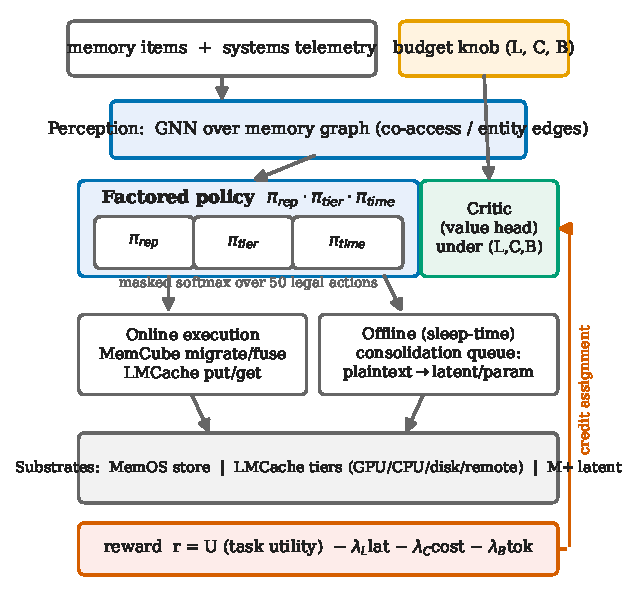
\includegraphics[width=\columnwidth]{fig_architecture.pdf}
  \caption{The STOA control plane. A GNN perceives the memory graph; a factored, masking-exact policy and
  a budget-conditioned critic emit one action per item; online and sleep-time branches execute against the
  underlying store, tiers, and latent path. Task-utility reward flows back through credit assignment.}
  \label{fig:arch}
\end{figure}

\paragraph{Perception.}
A graph network encodes the memory store as a graph whose nodes are items and whose edges are co-access
and entity links, together with per-tier occupancy telemetry, into a per-item embedding. Acting on the
whole batch through a graph network---rather than scoring items independently---lets co-accessed items
inform one another's placement and avoids per-item combinatorics, following Decima's use of a GNN for
scheduling~\cite{S5_mao2019decima}.

\paragraph{Policy.}
A factored actor emits the three decisions $(\rho,\tau,t)$ per item through separate representation, tier,
and timing heads, combined and softmaxed over exactly the 50 legal joint actions so masking is exact
(\Cref{sec:formulation}). A constrained critic---a value head---estimates the value of a placement under
the current budget $(L,C,B)$ and serves as the baseline for policy-gradient updates. A separate
admission/consolidation head selects which items enter the sleep-time queue for offline promotion.

\paragraph{Execution.}
Online actions are executed inline on the serving path as MemCube migrate/fuse operations and LMCache
put/get calls. Offline (sleep-time) actions run during idle windows: promoting plaintext to latent or
parameter forms, or summarizing a cluster of turns into a graph, amortized off the serving
path~\cite{F4_fang2025lightmem,F3_lin2025sleeptime}.

\paragraph{Credit assignment.}
The hard part is that a placement's payoff arrives many steps later---at query time---and memory edits
fracture the trajectory prefix, so naive policy gradients are high-variance and biased. STOA combines
three ingredients: (a)~\textbf{Belady-oracle imitation}~\cite{S2_liu2020parrot} to warm-start the policy
from hindsight-optimal placements computed offline from full future access traces; (b)~\textbf{process
supervision} with a learned critic that assigns dense, step-level rewards to migration and consolidation
actions~\cite{F20_xiong2025raggym}; and (c)~\textbf{segment-level advantages} over the trajectory segments
induced by memory edits~\cite{F7_zhang2025memoryasaction}. Training proceeds offline-RL first---safe on
logged traces, in the style of production cache-eviction RL~\cite{S4_coldrl2025}---and then guarded online.
\textbf{None of this machinery is evaluated in this paper.} \Cref{sec:evidence} measures the decision
the architecture would make --- whether a better belief about which items will be reused buys a better
placement --- and finds that it does not. We therefore report the formulation and the measurement, and
leave the policy itself as a design that our own evidence does not currently motivate building.

\section{What Placement Has To Get Right}
\label{sec:evidence}

\Cref{sec:formulation} frames placement as a learnable budget-constrained MDP. This section reports what
we found when we tried to learn it on production KV traces, and it is organized around a defect rather
than a result, because the defect came first and everything else follows from it: the protocol these
studies use --- ours for three revisions --- makes 97\% of the achievable benefit unreachable, so a
policy measured inside it looks flat however well it ranks (\Cref{sec:reachable}). Moving the decision to
each block's arrival recovers the benefit, and shows that the recoverable part is captured by
\emph{deciding early} rather than by \emph{deciding well} (\Cref{sec:arrival}). We then report what a
better ranker buys once the metric is repaired (\Cref{sec:capacity}), where reaction stands
(\Cref{sec:reaction}), and --- at length, because it is the most transferable part --- the protocol,
including the three claims we retracted along the way (\Cref{sec:protocol}).

\subsection{Sources and references}
\label{sec:sources}
We use \textbf{Mooncake}~\cite{qin2024mooncake}, replayed production traces from a general LLM serving
stack (23{,}608 and 12{,}031 requests), and \textbf{kv-cache-tester}, anonymized agentic coding
conversations (200 of 739 fetched). Each request lists the hash ids of the KV blocks it touches, so a
repeated hash is a genuine reuse. Both sources record wall-clock request timestamps. Block ids in
kv-cache-tester are conversation-scoped, so we namespace them before pooling; not doing so invents
cross-conversation reuse.

Three references bound every policy, all billed on the true future: a \textbf{hindsight oracle} that ranks
and places knowing future access counts; a \textbf{frequency heuristic} that assumes the future looks like
the observed prefix; and a \textbf{naive} all-plaintext baseline. ``Headroom'' is
$(\text{cost}_{\text{heur}} - \text{cost}_{\text{oracle}})/\text{cost}_{\text{heur}}$; ``captured'' is the
fraction of that interval a learned policy recovers.

\subsection{The protocol decides what is reachable}
\label{sec:reachable}
Placement studies of this kind fix a \emph{split instant}: observe the trace up to some point, build
features from that prefix, place every block, and bill the result against what the future turns out to
contain. It is the natural protocol, it is what we ran for three revisions of this paper, and it has a
structural defect that no aggregate computed inside it can reveal.

The defect is general, not particular to our setup. Whenever a workload admits new items after the split
--- which is to say, whenever it is not a closed working set --- a split-time policy has no opinion about
those items while the hindsight oracle it is scored against ranks them freely. The reported ``fraction of
headroom captured'' then divides by a quantity that is partly unreachable, and the unreachable share
grows with the arrival rate. Any study reporting that fraction without bounding it is reporting a number
whose denominator it has not characterized.

Feature construction can only describe a block that has been seen. On these traces
\textbf{45.2\% and 46.1\% of blocks have no pre-split access at all}, and a policy therefore has no
opinion about them --- but the hindsight oracle it is scored against ranks them anyway, using knowledge
of a future in which they exist. Those blocks carry \textbf{96.9\% and 97.6\%} of the oracle's total
advantage. The denominator of every ``captured headroom'' number we reported was, in other words,
almost entirely unreachable by construction:

\begin{center}\small
\begin{tabular}{@{}lrr@{}}
\toprule
& conversation & toolagent \\
\midrule
blocks with no pre-split access & 45.2\% & 46.1\% \\
full hindsight gap & 160{,}200 & 162{,}602 \\
\textbf{attainable gap} (clairvoyance on visible blocks) & \textbf{4{,}996} & \textbf{3{,}900} \\
share of the gap a causal policy cannot reach & \textbf{96.9\%} & \textbf{97.6\%} \\
\bottomrule
\end{tabular}
\end{center}

\medskip
\noindent A policy confined to 3\% of the prize will look flat no matter how well it ranks, and that is
what our earlier ``decoupling'' result measured. We retract it (\Cref{sec:protocol}).

\paragraph{The diagnostic is one line.} Compute the oracle's advantage twice --- once with clairvoyance
over every item, once restricted to the items the policy could have had an opinion about --- and take the
ratio. If it is far from one, the protocol is the finding. It costs a single extra placement pass, it
needs no new data, and running it on the first day would have saved this paper three revisions. We ship
it as \texttt{attainable\_ceiling} in the artifact and recommend it as a standard reporting requirement
for placement and admission studies: \emph{state the reachable share alongside any captured fraction}.

\subsection{Deciding on arrival, not at a split}
\label{sec:arrival}
The 97\% lives in blocks that do not exist yet when a split-time policy decides. The fix is not a better
model but an earlier decision: place each block \emph{when it first appears}, from context available at
that instant --- the shared-prefix session's age, request rate and recency, the block's position within
its request, the request's length. No feature reads the future; the model is fitted on the first half of
arrivals in arrival order and places the second half.

\begin{center}\small
\begin{tabular}{@{}llrrr@{}}
\toprule
trace & arm & AUC & of full gap & of attainable \\
\midrule
conversation & arrival-learned  & 0.574 & 82.8\% & 91.6\% \\
             & \textbf{arrival-FCFS} & 0.500 & \textbf{84.2\%} & \textbf{93.2\%} \\
             & arrival-shuffled & 0.500 & 82.6\% & 91.4\% \\
             & ceiling          & 1.000 & 90.4\% & 100.0\% \\
\midrule
toolagent    & arrival-learned  & 0.635 & 47.0\% & 88.9\% \\
             & \textbf{arrival-FCFS} & 0.500 & \textbf{47.3\%} & \textbf{89.5\%} \\
             & arrival-shuffled & 0.500 & 45.8\% & 86.6\% \\
             & ceiling          & 1.000 & 52.8\% & 100.0\% \\
\bottomrule
\end{tabular}
\end{center}

\medskip
\noindent Three readings, in order of how much they change the design question.

\emph{Timing recovers the benefit.} The reachable share rises from 3.1\% to \textbf{90.4\%} on
conversation and 2.4\% to \textbf{52.8\%} on toolagent --- $29\times$ and $22\times$. The headroom was
never absent; the protocol could not reach it.

\emph{Deciding at all captures almost all of it; deciding well adds nothing.} First-come-first-served
admission with a fixed action reaches 93.2\% and 89.5\% of the ceiling. The learned arm, at AUC 0.574
and 0.635, reaches 91.6\% and 88.9\% --- \emph{slightly worse}. We are not claiming the learned arm is
harmed by learning; at these AUCs the ranking is close enough to noise that spreading beliefs across the
per-item cost function's thresholds costs more than the ordering wins.

\emph{Even the ordering barely matters.} Shuffling the arrival order costs 1.8 and 3.0 points. What is
left --- the overwhelming majority --- is attributable to nothing more than making the decision at the
moment the block appears.

The design implication is the one the earlier framing could not reach: on these workloads, build an
\textbf{admission point}, not a predictor. That is also where the caching literature has been pointing.
Baleen~\cite{S12_wong2024baleen} is the one system among those we survey that decides admission rather
than eviction, and it optimizes a downstream system cost rather than miss rate.

\subsection{What a better ranker buys, once the metric is fixed}
\label{sec:capacity}
The capacity ladder of our earlier draft asked whether a stronger model converts into a better placement.
Under the corrected metric --- ties broken by tier speed rather than enum order, and every belief
quantile-matched onto one magnitude multiset so that only the ordering varies --- the answer is that
ranking quality moves the outcome monotonically and never enough to help:

\begin{center}\small
\begin{tabular}{@{}lrrr@{}}
\toprule
rung & AUC (conv / tool) & \% of attainable (conv) & (tool) \\
\midrule
constant        & 0.50 / 0.50 & $-154.6$ & $-825.7$ \\
random          & 0.49 / 0.50 & $-208.2$ & $-838.6$ \\
$\log$(count)   & 0.64 / 0.71 & $-70.9$  & $-75.8$ \\
logistic        & 0.81 / 0.93 & $-18.8$  & $-32.1$ \\
GBDT            & 0.80 / 0.91 & $-23.9$  & $-33.0$ \\
MLP             & 0.82 / 0.93 & $-8.5$   & $-19.3$ \\
\midrule
ceiling         & 1.00        & $100$    & $100$ \\
\bottomrule
\end{tabular}
\end{center}

\medskip
\noindent The damage falls monotonically as AUC rises ($-154 \to -71 \to -19 \to -8.5$), so ranking
quality does convert --- into less harm. Every arm is nonetheless below the frequency baseline, because
forcing an imperfect ranking onto the oracle's magnitude multiset assigns large beliefs to blocks that
will not be reused.

\paragraph{The magnitude convention decides the sign, and we measured by how much.}
We report the table above under a stated convention because it does not survive an unstated one. Running
each rung twice --- once on the scale its own scores naturally produce, once quantile-matched onto a
common multiset, \emph{with the ordering identical in both} --- gives:

\begin{center}\small
\begin{tabular}{@{}llrrr@{}}
\toprule
trace & rung & native scale & common scale & difference \\
\midrule
conversation & logistic & $+75.0$ & $-18.8$ & 93.8 \\
             & $\log$(count) & $-39.2$ & $-70.7$ & 31.5 \\
             & random   & $-81.1$ & $-208.2$ & 127.1 \\
\midrule
toolagent    & logistic & $+84.8$ & $-32.1$ & 117.0 \\
             & $\log$(count) & $-25.2$ & $-59.1$ & 33.9 \\
             & random   & $-630.2$ & $-838.6$ & 208.5 \\
\bottomrule
\end{tabular}
\end{center}
\noindent{\footnotesize Percent of the attainable ceiling. The two columns differ only in the magnitudes
attached to an identical ranking.}

\medskip
\noindent The same policy, with the same ordering, scores $+84.8\%$ or $-32.1\%$ depending on a choice
of scale. The gap runs from \textbf{31.5 to 208.5 points} --- an order of magnitude larger than any
effect this paper or its predecessors reported. An earlier draft asserted that this control ``changes
the captured headroom by about two points''; that number was never computed, and it is wrong by two
orders of magnitude.

We therefore claim neither column. What we do claim is the comparison \emph{within} a column, which is
well defined: on the common scale, ranking quality converts monotonically into less harm. And we claim
the methodological point, which we think is the more useful one: \textbf{``fraction of headroom
captured'' is not a quantity until the magnitude convention is stated}, and no version of this paper,
nor any placement study we are aware of, states it.


\begin{table}[t]
  \centering \small \setlength{\tabcolsep}{4pt}
  \begin{tabular}{@{}lrr@{}}
    \toprule
     & \makecell{Mooncake\\(serving)} & \makecell{kv-cache-tester\\(agentic)} \\
    \midrule
    requests analysed              & 23{,}608 / 12{,}031 & 4{,}215 (40 conv.) \\
    blocks touched exactly once    & 78\%   & 15\% \\
    mean reuse per block           & 1.9    & 24 \\
    blocks per request             & $\sim$17 & $\sim$1{,}900 \\
    block size (tokens)            & 256    & 64 \\
    \midrule
    headroom, heuristic vs.\ oracle & 87\%  & 81--94\% \\
    headroom captured by a learned policy & $+2$\% & not measurable$^\dagger$ \\
    \bottomrule
  \end{tabular}
  \caption{The two sources, at the scales actually analysed. Descriptive statistics are
  sample-dependent: the agentic figures shift with the number of pooled conversations (one-time fraction
  ranges 7.5--21\% over 20--200 conversations), and the captured-headroom range spans a sign reversal
  between 40 and 150 conversations (\Cref{sec:protocol}). We report the spread rather than a point
  because the sampling is not randomized. $^\dagger$Under randomized draws the agentic figure has a 95\%
  spread an order of magnitude wider than any effect (\Cref{sec:sampling}).}
  \label{tab:regimes}
\end{table}


\subsection{A measurement that was never a measurement}
\label{sec:sampling}
We also attempted the obvious follow-up --- fit a richer per-block model on the agentic source and place
with it --- and first obtained what looked like a strong positive: $+66$ to $+88\%$ of the headroom
captured, reproducing across what we took to be two samples. It was not a result, and the way it failed is
worth more than the number would have been.

The two samples were \emph{sorted prefixes} of the conversation corpus, so the smaller was contained in
the larger; and file index correlates strongly with conversation shape (mean requests per conversation
falls from 140 to 37 between files 1--20 and 71--150). Extending the same prefix to 100 and 150
conversations drove the captured headroom to $-9\%$ and $-48\%$ --- a sign reversal. Re-drawing the
samples \emph{at random} rather than as prefixes then showed why: four random draws at 40
conversations land between $-234$ and $+66$ points, and at 20 conversations between $-1207$ and $+78$
(\Cref{tab:kvct}). The spread dwarfs the effect by an order of magnitude. We quote the observed range
rather than a confidence interval on purpose: with four draws a parametric interval rests on a normality
assumption these data cannot support, and \emph{captured} is a ratio whose denominator varies per draw.
An earlier revision of this paper reported $\pm126$ here, computed with the normal quantile against a
standard deviation estimated from four points; the correct $t(3)$ half-width is $\pm205$. That error is
the eleventh entry in \Cref{sec:protocol}'s catalogue and it was ours. Under a correct sampling protocol there was never a
measurement here to report.

We keep this in the paper for two reasons. It is the control that our own protocol
(\Cref{sec:protocol}) lacked, and running it costs minutes; and it bounds what the rest of our numbers
are worth, since every other result in this section is also a single draw of a parameter we chose.

\begin{table}[t]
  \centering \small \setlength{\tabcolsep}{5pt}
  \begin{tabular}{@{}lcc@{}}
    \toprule
    & \makecell{sorted-prefix samples\\(as first reported)} & \makecell{4 random draws\\mean [observed range]} \\
    \midrule
    20 conversations & --- & $-541\%$ $[-1207, +78]$ \\
    40 conversations & $+88\%$ & $-67\%$ $[-234, +66]$ \\
    70 conversations & $+87\%$ & --- \\
    100 conversations & $-9\%$ & --- \\
    150 conversations & $-48\%$ & --- \\
    \bottomrule
  \end{tabular}
  \caption{Headroom captured by a learned placement policy on agentic traces, the same pipeline measured
  two ways. Left: sorted-prefix samples, which are nested and drawn from a corpus whose per-conversation
  statistics vary threefold along the file index --- the numbers we first reported, and their reversal.
  Right: randomized draws at the same sizes, summarized by their observed range --- four draws cannot
  support a parametric interval. The spread is an order of magnitude wider than any effect, so this
  quantity was never measurable under this protocol. We report it as a cautionary measurement.}
  \label{tab:kvct}
\end{table}


\subsection{Where reaction stands}
\label{sec:reaction}
If forecasting does not pay, the alternative is to react. On the full Mooncake traces, reactive tiering
reaches 75--99\% of Belady's hit rate on the toolagent trace and 40--94\% on open-ended conversation
using LRU, LFU or a fill-once cache alone; admitting the adaptive and learned policies below widens the
per-operating-point envelope only to 76--99\% and 42--94\% (\Cref{fig:reactive}).

The interesting question is not the envelope --- that is an oracle over policies, not something anyone
deploys --- but whether any \emph{single} policy attains it, and whether the adaptive designs built for
exactly this situation beat plain rules. We therefore run the family: \textbf{ARC}~\cite{S7_megiddo2003arc},
which shifts a recency/frequency split on ghost hits; \textbf{LeCaR}~\cite{S8_vietri2018lecar} and
\textbf{CACHEUS}~\cite{S9_rodriguez2021cacheus}, which replace ARC's arithmetic update with regret-based
multiplicative weights over two experts; and the learned \textbf{LRB}, which is reported separately below because its
numbers carry an implementation band the others do not.

\begin{center}\small
\begin{tabular}{@{}lrrrrr@{}}
\toprule
trace & tier & best pure & ARC & LeCaR & CACHEUS \\
\midrule
conversation & 2\%  & 39.8 & 29.4 & \textbf{42.3} & 35.9 \\
             & 5\%  & 53.3 & \textbf{57.9} & 56.8 & 53.5 \\
             & 10\% & 76.0 & \textbf{77.5} & 77.2 & 75.3 \\
             & 20\% & \textbf{94.1} & 87.4 & 93.9 & 88.8 \\
\midrule
toolagent    & 2\%  & 74.9 & 70.7 & \textbf{75.8} & 73.9 \\
             & 5\%  & 81.3 & \textbf{83.6} & 83.0 & 82.9 \\
             & 10\% & 91.9 & 92.3 & \textbf{92.9} & 91.8 \\
             & 20\% & 99.3 & 96.3 & \textbf{99.3} & 97.6 \\
\bottomrule
\end{tabular}
\end{center}
\noindent{\footnotesize Percent of Belady's hit rate. ``Best pure'' is the better of LRU, LFU and a
fill-once cache at that operating point.}

\medskip
\noindent Across eight operating points and four designs, \textbf{the best adaptive or learned policy
beats the best pure rule by at most 4.6 points of Belady}, and at two points by nothing at all. Which
design wins also moves: LeCaR at the tightest tier on both traces, ARC in the middle, plain LRU at the
loosest. That is the substantive finding --- not that these policies fail, but that on KV-block workloads
the whole adaptive-replacement family collapses into a band a few points wide, well short of the oracle
at the small tiers where the decision actually matters.

The diagnostics say why, and the reason is specific to KV workloads. Every policy in this family adapts
on a \emph{ghost hit} --- a miss on a block it recently evicted --- whether it updates a split (ARC) or
an expert weight (LeCaR, CACHEUS). But 76--78\% of blocks in these traces are never reused at all, so
most evictions are correct and produce no signal. Measured, ARC receives an adaptation signal on
\textbf{3.5--7.3\% of misses}; the regret-based policies read the same channel, which is why they land
in the same band rather than above it. What signal it does get is not merely sparse but, at
the smallest tier, directionally wrong: at a 2\% tier ARC drives $p$ to 90\% recency on both traces, while
the rule that actually wins there is frequency. A workload whose blocks are mostly singletons starves the
very mechanism adaptive replacement runs on.

\paragraph{And the learned cache policy loses to both --- but only as a range.} The strongest
counter-argument to this paper is LRB~\cite{S6_song2020lrb}, which learns a relaxed-Belady objective from
a far richer feature set than our four trace-local statistics and won on production CDN traces. We
reimplement it: GBDT regression on log time-to-next-request over inter-access deltas and exponentially
decayed counters, sampled eviction, online retraining from a sliding memory window, right-censored
labels.

Our first version of it measured something else entirely. The training buffer was capped by truncating to
its tail; labelled rows arrive one at a time as blocks are re-accessed while censored rows arrive in one
contiguous burst per checkpoint, so from the third retrain onward every training label was identical, the
regressor returned a constant, and eviction degenerated to a uniform draw over the sampled candidates.
A random-replacement control reproduces that column to within 1.5 points at all eight operating points.
We report the repaired numbers and, because two defensible repairs disagree, we report them as a band:

\begin{center}\small
\begin{tabular}{@{}lrrrr@{}}
\toprule
trace & tier & LRB (repaired) & ARC & below ARC? \\
\midrule
conversation & 2\%  & 27.6--29.2 & 29.4 & yes \\
             & 5\%  & 30.9--32.2 & 57.9 & yes \\
             & 10\% & 45.0--45.9 & 77.5 & yes \\
             & 20\% & 75.8--76.5 & 87.4 & yes \\
\midrule
toolagent    & 2\%  & 68.8--69.0 & 70.7 & yes \\
             & 5\%  & 71.1--71.4 & 83.6 & yes \\
             & 10\% & 80.9--83.0 & 92.3 & yes \\
             & 20\% & 94.6--94.9 & 96.2 & yes \\
\bottomrule
\end{tabular}
\end{center}
\noindent{\footnotesize Percent of Belady. The band spans two repairs of the truncation bug: subsampling
all accumulated rows, and dropping rows older than the memory window first. We adopt the second, which is
what a ``sliding memory window'' means.}

\medskip
\noindent \textbf{The band understates the uncertainty.} An independent reimplementation of the same
repair, produced during review of this paper, reports $\approx$63\% at conversation/10\% where ours gives
45.9\%. We cannot reconcile a 17-point difference without that code. So the honest reading is that our
LRB \emph{point} estimates are not citable to better than about twenty points --- wider than several
differences this paper's earlier drafts drew conclusions from. What survives that band is the ordering:
\textbf{LRB is below ARC at all eight operating points under every repair we or the reviewer produced,
including the 63\% reading.} That is the claim we make; the numbers are context for it.

The mechanism appears to be the one that limits ARC, seen from the other side. LRB learns from labels the
trace supplies when a sampled block is requested again; a block that never returns yields a
\emph{right-censored} row, which says only ``not within the window'' and nothing about when. At the
default window \textbf{77--83\% of LRB's training rows are censored}, and 86--89\% at a shorter one. A
population dominated by singletons starves the ghost-hit channel that adaptive replacement runs on and
the regression target that learned replacement runs on, for the same underlying reason.

Three caveats bound this. It is our reimplementation of the published mechanism, not the authors'
artifact. KV blocks are uniform-size, so byte miss ratio collapses to object miss ratio and LRB loses one
of its structural advantages over LRU. And the hyperparameter sweep we ran to check that the result was
not a tuning artifact was run on the \emph{broken} implementation, so it tested the robustness of random
eviction; we have not repeated it.


The eviction signal also inverts by source. On the agent traces LRU reaches 0.88--0.95 of Belady at a 5\%
tier while LFU stays near 0.23--0.27; on Mooncake the ordering reverses below the working-set knee. An
eviction policy tuned on one source is a poor default for the other --- and, as both the ARC and the LRB
result show, reaching for a more sophisticated policy does not by itself resolve the choice.

\begin{figure}[t]
  \centering
  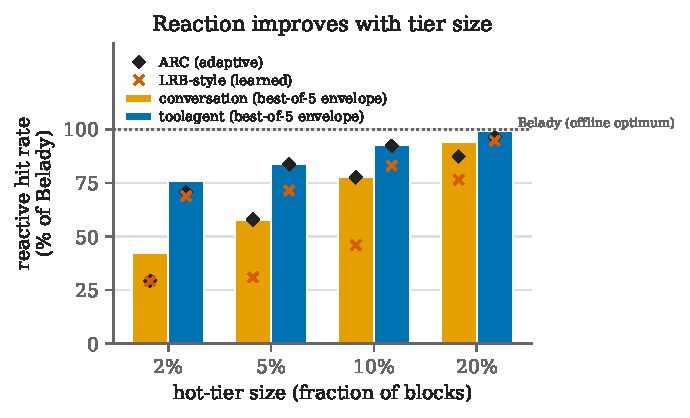
\includegraphics[width=\columnwidth]{fig_reactive.pdf}
  \caption{Reactive tiering as a fraction of Belady's hit rate, full Mooncake traces. Bars are a
  per-operating-point best-of-five envelope, an oracle over policies rather than a policy. Diamonds are
  ARC, which meets the envelope at 5\% and 10\% but falls short at both extremes; crosses are the
  LRB-style learned policy, which is below ARC everywhere.}
  \label{fig:reactive}
\end{figure}

\subsection{Placement is not retrieval}
\label{sec:placement-vs-retrieval}
A tiering scheduler decides what to keep hot; a retriever decides what enters the prompt. Our first
attempt to measure the difference on LoCoMo~\cite{P51_maharana2024locomo} resolved nothing: two runs
ranked the arms oppositely, and across nine comparisons in each, not one survived correction for
multiplicity. A power analysis said why --- separating the query-agnostic arms needed 246--710 scored
questions per arm and we had 30 --- and also said the reversal was not small-sample noise but came from
the two runs drawing \emph{different dialogues}, which is \Cref{sec:sampling}'s failure in a different
corpus.

We therefore re-ran it at the size the analysis asked for: all ten released dialogues, 30 held-out
questions each, \textbf{300 scored questions per arm}, LLM-judged. Because every arm answers the same
questions the comparison is paired, so we test it with McNemar on the discordant pairs rather than
Fisher on independent samples, and report a per-dialogue sign test alongside so a result cannot rest on
one dialogue.

\begin{center}\small
\begin{tabular}{@{}rrrrr@{}}
\toprule
budget & demand & random & centrality & retrieval \\
\midrule
10\% & 12.0 & 6.7 & 1.7 & \textbf{51.7} \\
25\% & 16.7 & 11.3 & 6.3 & \textbf{52.7} \\
50\% & 29.3 & 25.3 & 16.3 & \textbf{55.3} \\
\bottomrule
\end{tabular}
\end{center}
\noindent{\footnotesize QA accuracy (\%), 300 questions per cell. The first three arms are
query-agnostic placement; retrieval sees the question and is therefore better informed by construction.}

\medskip
\noindent \textbf{Six of the nine comparisons now survive Bonferroni correction}, where none did before.
That is three distinct claims, each replicated at three nested budgets over the same 300 questions, not
six independent findings --- and Bonferroni is the right correction precisely because those tests are
dependent, since it controls the family-wise error rate under arbitrary dependence. Holm on the same
nine $p$-values rejects the same six.

\emph{Retrieval dominates placement, decisively.} It leads at every budget, by a factor of four at the
tightest one, with $p < 10^{-15}$ and the same direction in \textbf{10 of 10 dialogues} (sign test
$p = 0.002$). What was previously argued from scoping is now measured: a query-aware retriever and a
query-agnostic placement policy are not competing for the same job, and a placement signal evaluated as
if it were a retrieval signal will always look bad.

\emph{The placement signal is nonetheless real within its own regime.} Ranking turns by evidence demand
beats embedding centrality --- the fair same-regime baseline --- at every budget ($p \le
1.2\times10^{-4}$). At the dialogue level it leads in 8, 10 and 9 dialogues of 10 (sign test $p = 0.008$,
$0.002$, $0.022$); two of those three do not clear the corrected threshold on their own, so the
question-level test is doing the work here. Query-agnostic placement is not noise; it is simply solving a different and
strictly harder problem than retrieval, with no access to the query.

\emph{One comparison is still unresolved, and we say by how much.} Demand versus random selection points
the right way at all three budgets but reaches only $p = 0.029$, $0.068$ and $0.256$, and at the
dialogue level says nothing at all (5--2, 6--2 and 7--3 dialogues; sign test $p = 0.45$, $0.29$, $0.34$).
At the observed discordance rates, 80\% power would need \textbf{758, 1078 and 2589 questions per arm}
at the corrected threshold we judge significance against --- 486, 667 and 1593 if one sizes at an
uncorrected $0.05$, which is the mistake an earlier revision of this paper made. Against the 300 we ran,
the shortfall is between $2.5\times$ and $8.6\times$. We report this as open with its sample size
attached rather than as a null, and note that a required $n$ estimated from the same data whose null it
describes is itself a noisy quantity: across seeds it moves by roughly 10\%.

The reading we take from this is scoping, now with evidence behind it: placement governs latency and
cost, retrieval governs which facts reach the model, and the two compose rather than compete.


\subsection{The representation axis, and what it says about our own formulation}
\label{sec:representation}
\Cref{sec:formulation} decides representation jointly with tier because the two are argued to be
coupled: a compressed item is cheap to serve but may cost accuracy, so the right form depends on the
budget. Every experiment above holds representation at plaintext, which means that argument --- the
reason the joint decision exists --- had never been tested. We test it here, on LoCoMo, with the same
fact ids, questions and gold answers under three representations that differ only in text and token
cost: the turn verbatim, an LLM summary, and an aggressive key--value extract. All three are
\emph{textual}; the vector, graph, latent and parameter forms of \Cref{sec:formulation} are not
instantiated anywhere in this work, so what follows probes the axis rather than exercising it. Budgets are a fraction of
the \emph{plaintext} total for all three, so a compressed form is not quietly handed a larger allowance.

\begin{center}\small
\begin{tabular}{@{}rrrr@{}}
\toprule
budget & plaintext & summary & extract \\
\midrule
5\%  & 5.0  & \textbf{11.0} & 5.0  \\
10\% & 10.0 & \textbf{15.0} & 7.0  \\
25\% & 19.0 & \textbf{26.0} & 21.0 \\
50\% & 32.0 & \textbf{38.0} & 22.0 \\
\bottomrule
\end{tabular}
\end{center}
\noindent{\footnotesize QA accuracy (\%), 100 questions per cell, LLM-judged. Mean compression ratio:
summary $0.58\times$, extract $0.19\times$.}

\medskip
\noindent Two things are visible and one is not. The trade-off the formulation posits is \emph{visible}:
compress far enough and utility appears to collapse, with the $0.19\times$ extract ten points behind
plaintext at the loosest budget --- though that gap, like everything else here, clears no significance
threshold. But the optimum \emph{does not move}. Summary leads at all four budgets, with the
discordant pairs favouring it every time (6--0, 5--0, 11--4, 19--13). If that holds, representation on
this workload need not be re-decided per operating point --- a weaker coupling than we assumed when we
wrote \Cref{sec:formulation}.

What is not visible is significance. \textbf{None of the eight comparisons survives correction} (best
raw $p = 0.031$ against a 0.00625 threshold); at the observed discordance rates, resolving
summary-versus-plaintext needs 188--1138 questions per cell at the corrected threshold (129--718 at an
uncorrected $0.05$) against the 100 we ran. By the rule we impose
on ourselves in \Cref{sec:protocol}, this is a direction with a sample size attached, not a result. We
report it because it is the first time the axis has been exercised at all, and because the direction
points against our own framing rather than for it.


\subsection{What the measurement required}
\label{sec:protocol}
Every positive result we obtained before the final protocol was an artifact. We report the mechanisms
because they generalize, and because the last three were found only by adversarial review rather than by
our own checks.

\paragraph{Reference-frame mismatches (six).} Two quantities that must share a frame --- the same split
instant, ordering, tie rule, or question set --- were silently defined on different ones: a demand signal
computed from the questions being scored; policy features derived from whole-trace access counts; an
oracle that inherited the heuristic's ordering and so showed zero headroom; a train/test split taken over
access-event indices rather than time, which on real traces falls past the end of the trace; a ranking
metric that broke ties by label, inflating a raw count feature from AUC 0.51 to 0.94; and features built
at one split instant while costs were billed at another.

\paragraph{Retracted claims (three).} Each survived our own checks and was found later --- the last two
by adversarial review, after the catalogue below had already been written. \textbf{(i)} A headline
``+66--88\% of headroom captured on agentic traces'' that reversed sign at a larger sample and that
randomized draws showed had never been measurable (\Cref{sec:sampling}). \textbf{(ii)} A
\emph{decoupling} claim --- prediction improves while placement does not --- that was an artifact of
normalizing against an oracle ranking blocks a causal policy cannot see (\Cref{sec:reachable});
normalized against what is attainable, ranking quality converts monotonically. \textbf{(iii)} A reported
LRB column that measured \emph{random eviction}: the training buffer was truncated to its tail, censored
rows arrive in one contiguous burst per checkpoint, and from the third retrain onward every training
label was identical, so the regressor returned a constant and eviction degenerated to a uniform draw.
Two independent repairs of that bug disagree by 19 points, so we withhold the column rather than publish
either.

The common shape is worth naming: in all three the \emph{aggregate looked reasonable}. A flat captured
fraction, a plausible interval, a learned policy landing below ARC --- each is what the hypothesis
predicted, and none of our checks compared the quantity against what it was arithmetically able to be.

\paragraph{Free-parameter extrapolations (three).} Each was a curve read from one point, in a parameter
fixed for convenience. A reactive claim taken at a single cache size reversed under a sweep. A headroom
taken at 6\% of the trace moved six points by full length (81.0\% to 87.2\%), and the placement
benefit read off it peaked mid-sweep rather than at the longest trace. And a learned-placement result taken at 40 and
70 conversations --- \emph{nested prefixes} of a corpus whose per-conversation statistics vary threefold
along the file index --- reversed sign at 150, from $+88\%$ to $-48\%$, and took a headline claim with it.

\paragraph{Believing a report over an observation (one).} An edit script targeted a heading an earlier
revision had removed, matched nothing, and printed success anyway.

\paragraph{The controls.} Assert that the oracle beats the heuristic it is compared against; keep a
no-learning baseline of the same functional form as the learned one; check that no single feature
outperforms the fitted model; before concluding that a signal is unlearnable, vary model capacity while
holding the protocol fixed, so ``the model was too weak'' is excluded rather than assumed
(\Cref{sec:capacity}); compare reference frames explicitly rather than trusting that two code paths
agree; verify an edit landed rather than that it reported success; sweep every parameter chosen for convenience
before stating a result that depends on it --- the one we lacked; and, before reporting any null, compute
the sample size that would have resolved it, because ``we could not tell'' and ``there is nothing there''
are different claims and only the first is ours to make. The harness ships with all of these wired in,
and a checker that re-derives every number in this paper from its artifact and fails if the two have
drifted --- which caught four rounding drifts and one claim that had quietly mixed two hyperparameter
settings.

\subsection{Limitations}
\label{sec:limits}
No real vLLM+LMCache deployment was measured, so any cost-expressed quantity should be read as a range.
We tightened what that range means. Our first sensitivity analysis scaled every tier latency by a common
factor, which moves the absolute scale and leaves the \emph{ratios} between tiers untouched --- and the
ratios are what a placement policy responds to, so it never tested the parameter that mattered. We
therefore derive the table instead: KV bytes per block follow exactly from a model's attention shape
($2 \times \text{layers} \times \text{kv\_heads} \times \text{head\_dim} \times \text{dtype}$ per
token), and per-tier latency is that divided by a declared device-class bandwidth plus a fixed overhead.
Sweeping three attention shapes against five device classes puts headroom at \textbf{64--88\%}, which
contains the 81\% our hand-written table gives --- the conclusion survives, but two things about the
table do not. Its GPU:CPU latency ratio is 1:10 where the derivation gives 1:80 to 1:250, an order of
magnitude in the ratio the policy is most sensitive to; and \textbf{6 of the 15 device classes reorder
the hierarchy} so that latency order and capacity order disagree, which our fixed per-tier capacity table
cannot express at all. Calibrating against a live deployment remains the open gate; this is the honest
intermediate, not a substitute. The
\emph{timing} axis of \Cref{sec:formulation} is not exercised at all, and the \emph{representation} axis
only as the underpowered pilot of \Cref{sec:representation}; neither is touched by the KV traces. Both
sources are KV-block hash streams from transformer prefix caching, so they are independent in provenance
but not in mechanism; with one exemplar per putative regime we cannot separate workload character from
vendor, date, or block size (256 vs.\ 64 tokens). Sampling is not randomized and no confidence interval is
reported for the placement results, though the two remaining free parameters --- trace length and split
instant --- are now swept rather than fixed. Of the learned and adaptive cache literature we evaluate
ARC~\cite{S7_megiddo2003arc}, LeCaR~\cite{S8_vietri2018lecar}, CACHEUS~\cite{S9_rodriguez2021cacheus} and
a reimplementation of LRB~\cite{S6_song2020lrb}; Hawkeye, Mockingjay and Baleen are positioned in
\Cref{sec:related} but not run, the first two because a KV block hash carries no analogue of the program
counter their predictors are indexed by. Our LRB is the
published mechanism rebuilt from the paper, not the authors' artifact --- as are our LeCaR and CACHEUS, whose
CR-LFU expert we approximate by LFU --- and the uniform block size of both sources removes one of LRB's
advantages over LRU, so the underperformance we report should be read as a statement about this workload
rather than about these designs.

\section{Open Problems}
\label{sec:open}

Our result closes one question and sharpens several others.

\paragraph{What can a scheduler do that ordering cannot?}
\Cref{sec:arrival} shows that first-come-first-served admission captures 87.4\% of the reachable benefit
on conversation but only 50.2\% on toolagent, and that a learned ranker adds nothing on top of it on
either. So the recoverable benefit is not in per-item prediction. It is partly in \emph{when} the
decision is taken and partly --- on toolagent, worth 14 points --- in the order arrivals are admitted in,
which we do not currently model. What remains unclaimed on toolagent is large: half the reachable
benefit, and 81\% of the hindsight gap that arrival timing does not expose at all. Both have to come from
something the per-item formulation does not express: admission under contention, coordinated eviction
across concurrently-live sessions, or migration timed against idle windows. Identifying which of these
carries the gap, and building an evaluation that can see it, is the substantive next step, and it is a
scheduling question rather than a modelling one.

\paragraph{Calibration, and what a mis-specified cost model hides.}
Our tables are placeholders, and we saw concretely how misleading that is: under them the per-item optimal
action is identical for every reused block, which collapses a three-axis decision into a one-dimensional
sort and makes every policy look alike. Fitting the tables to a real vLLM+LMCache deployment --- the only
GPU-gated step in this work --- is a precondition for any claim about the representation and timing axes,
which our traces do not exercise at all.

\paragraph{Aggregate working set, not per-request footprint.}
Reactive sufficiency is governed by how much of the \emph{concurrently live} working set a tier holds, not
by one request's block count: holding tier size fixed in absolute blocks and raising the number of pooled
conversations still degrades the ratio. Characterizing that surface --- tier size against concurrency,
across sources --- would give an operator a sizing rule, which is the most directly actionable thing this
line of work could produce.

\paragraph{Composing placement with retrieval.}
\Cref{sec:placement-vs-retrieval} indicates the two are orthogonal in kind: placement sets latency and
cost, retrieval sets which facts reach the model. The open problem is the composition --- a retriever
running over a tiered store whose hot set a scheduler maintains, where a retrieval miss on a cold tier
costs latency rather than accuracy. Neither literature evaluates that joint object, and our own LoCoMo
measurement is far too small ($n=30$) to speak to it.

\paragraph{Sampling as a first-class experimental variable.}
Three of our ten defects were extrapolations from a single value of a parameter fixed for convenience, and
the most damaging reversed a headline claim's sign. For trace-driven work we would now require of
ourselves, and suggest for the area: randomized rather than prefix sampling, several disjoint draws with
intervals, and a reported sweep over every quantity the design fixes --- trace length, pool size, tier
size, split fraction --- before any claim that depends on one of them.

\paragraph{Safety and governance.}
A memory written by tools and other agents is an attack surface, and provenance must survive consolidation
so a fact can be traced, invalidated, or unlearned. A budget-constrained scheduler is a natural
enforcement point; doing that without giving back the frontier is unexplored.

\section{Related Work}
\label{sec:related}

We organize prior work by the three axes STOA unifies; \Cref{tab:positioning} summarizes which axis each
line decides and by what means.

\paragraph{Representation and memory-OS.}
MemOS~\cite{F1_li2025memos} and MemGPT~\cite{P14_packer2023memgpt} treat memory as an operating-system
problem, exposing abstractions (MemCube, virtual context) and primitives to migrate items between
plaintext, activation, and parameter forms; M+~\cite{F2_wang2025mplus} adds a co-trained latent memory.
These provide the \emph{mechanism} to change representation and tier but decide \emph{when} by heuristic;
STOA supplies the learned scheduler they lack.

\paragraph{Content and RL-based management.}
Memory-R1~\cite{F6_yan2025memoryr1} and Memory-as-Action~\cite{F7_zhang2025memoryasaction} learn, with
RL, \emph{what} to add, update, or delete and how to edit context, and the latter handles the
trajectory-fracturing that edits cause. But they operate over a single fixed representation and never
choose a physical tier or schedule offline consolidation---orthogonal to, and composable with, STOA.

\paragraph{Systems tiering and ML-for-systems.}
LMCache~\cite{F5_liu2025lmcache} tiers KV-cache bytes to cut miss-rate; H2O~\cite{S1_zhang2023h2o} evicts
by attention score. The learnability of such decisions is established: PARROT~\cite{S2_liu2020parrot}
imitates a Belady oracle for cache replacement, Cold-RL~\cite{S4_coldrl2025} does eviction with offline
RL in production, and Decima~\cite{S5_mao2019decima} schedules clusters with a GNN policy. STOA inherits
these techniques but changes the objective from miss-rate to downstream \emph{task utility}, and the
action from a single axis to the joint representation\,$\times$\,tier\,$\times$\,timing decision.

\paragraph{Offline consolidation.}
Sleep-time compute~\cite{F3_lin2025sleeptime} and LightMem~\cite{F4_fang2025lightmem} show the value of
precomputing and consolidating memory offline, but treat it as a global mode rather than a per-item,
budget-aware timing decision---the third axis STOA learns.

\paragraph{Learned and adaptive caching.}
Two lines bear directly on our results and we position against them explicitly, because our findings
reproduce rather than extend them. \textbf{LRB}~\cite{S6_song2020lrb} learns a relaxed-Belady objective
for CDN caching from a feature vector built out of the deltas between an object's past request
times --- the same family as the think-time features we tried here. Timing as a cache-scheduler input is
therefore established practice, not a new interface insight, and our (negative) placement result should
be read as a report that this family does not transfer to KV-block \emph{placement} under our cost model,
not as a novel signal. \textbf{ARC}~\cite{S7_megiddo2003arc} adaptively balances recency against
frequency precisely because neither dominates across workloads; the recency-versus-frequency inversion we
measure between our two sources (\Cref{sec:reaction}) is that observation restated on KV blocks, and an
adaptive policy of the ARC family is the baseline a deployment should reach for rather than either pure
rule.

The rest of the learned-cache literature divides by what it learns \emph{from} and what it decides, and
the division explains why our result is not a contradiction of it.
LeCaR~\cite{S8_vietri2018lecar} and CACHEUS~\cite{S9_rodriguez2021cacheus} learn no per-item model at all:
they run experts (LRU/LFU, and in CACHEUS scan- and churn-resistant variants) and update expert weights
from regret observed on a ghost list. That is the same evidence channel ARC uses, and
\Cref{sec:reaction} measures how thin it is here --- 3.5--7.3\% of misses carry any signal --- so the
family inherits the limitation rather than escaping it. We ran both to check, rather than leaving it as a
prediction, and both land in the same few-point band as ARC. LeCaR is nonetheless the best single policy
at the tightest tier on both traces, which is the one place the regret formulation visibly pays.
Hawkeye~\cite{S10_jain2016hawkeye} and Mockingjay~\cite{S11_shah2022mockingjay} are the closest
antecedents to what we attempted: both supervise a predictor with Belady replayed over history, Hawkeye
as a binary cache-friendly/averse label and Mockingjay as a multiclass reuse-distance estimate. They
operate at CPU last-level-cache granularity, where a program counter identifies a reuse pattern; a KV
block hash carries no analogous instruction identity, which is the structural reason their signal does
not simply port. Baleen~\cite{S12_wong2024baleen} is the one that decides admission and prefetching
rather than eviction, and the one that optimizes a downstream system cost (disk-head time) instead of
miss rate --- the closest precedent for the multi-objective reward of \Cref{sec:formulation}, and the
direction we think is right even though we do not evaluate it here.

Of these we evaluate LRB, LeCaR and CACHEUS (\Cref{sec:reaction}) --- and the prediction above is what we
measured: both expert policies land in the same few-point band as ARC rather than above it. Hawkeye,
Mockingjay and Baleen are positioned but not run.

In short, each line optimizes one axis and freezes the others, and none decides representation, tier,
\emph{and} timing jointly under a shared budget (\Cref{tab:positioning}). Our contribution is not a better
policy but a measurement: on production KV traces, ranking quality improves substantially while the
placement benefit it buys does not, and we report the protocol needed to see that.

\section{Conclusion}
\label{sec:conclusion}

For every item an agent remembers, three coupled questions---in what representation, on which tier, and
when to (re)materialize it---are today answered separately by three research communities. We gave a single
budget-constrained formulation that unifies them under one serve-time knob, and then asked whether the
resulting decision is learnable.

The answer is neither yes nor no but a decoupling, and that is the contribution. Reuse is predictable on
production traces and becomes more so with data, yet the placement benefit that predictability buys stays
near zero across the whole range; ordering, not calibration, is what the outcome turns on, and an oracle's
ordering would recover almost all of the gap. Reactive tiering, forecasting nothing, already delivers most
of the achievable benefit on one trace and rather less on the other, with the eviction signal itself
inverting between sources.

We arrived here only after removing ten measurement defects, each of which had
produced a plausible positive result; we report those mechanisms and the controls that catch them, because
the same traps are available to anyone measuring a memory scheduler. The useful next move is not a bigger model. It is to calibrate the cost
model against real tiers, to sweep the parameters an experiment fixes for convenience before believing any
result that depends on them, and to ask what a scheduler could do that ordering alone cannot. Agent memory
is ready to be scheduled---but first it has to be measured in a way that can tell schedulers apart.


\bibliographystyle{ACM-Reference-Format}
\bibliography{../docs/references}

\end{document}
